\chapter{Literature Review}
\label{chapter:background} 

In this chapter, the theoretical concept related to the subject of the study will be reviewed. We find it necessary to provide a general overview of machine learning, deep learning, and data augmentation as these concepts are the foundation stone of the thesis.


\section{Machine Learning}

Often machine learning and deep learning are used together to mean the same thing. However, there is a distinction between machine learning and deep learning. Machine learning is a broader set of automated learning tools which include deep learning as sub-field \citep{chollet2017deep}. Machine learning powers many aspects of modern life from simple web search to complex language translation. In a simple language, machine learning can be understood as a process where humans input data, as well as expected output from the data, then the machine produces the rules that match given input to its expected output \citep{chollet2017deep}. Expected output is optional as some machine learning problem do not have any expected output and the job of machine is to transform the input into a meaningful output. At the heart of the machine learning lies input data and a way to measure whether the rule learned by the machine is reliable or not \citep{chollet2017deep}. In this sense, the central problem of machine learning is to figure out the best possible transformation that provides the most accurate result. Sometimes this transformation is also referred to as representation. 

Machine learning task can be broadly classified into Supervised and Unsupervised learning. Supervised learning is the most common form of machine learning tasks. Like the majority of machine learning problems, the problem this thesis is trying to tackle also falls under supervised learning problem. Supervised learning problem is about learning to map input data to known targets also known as labels or annotations, given a set of examples \citep{chollet2017deep}. Most common application of deep learning such as image classification, speech recognition, and language translation falls under supervised learning. In this thesis, the problem is to map the spectral data in the form of arrays to its corresponding label of an organic compound. Unsupervised machine learning is the branch of machine learning that consist of finding the best representation or transformation of the input data without the help of any explicit expected output. Unsupervised machine learning are used for the purpose of data visualization, data compression, data denoising, or to better understand the correlations present in the data at hand \citep{chollet2015keras}.

To summarize, machine learning is an iterative process of finding the appropriate representation of input. It uses a feedback loop from the metric that determines the quality of representation and keeps iterating until it reaches the point where no further improvement of the metric is possible. 

\section{Deep Learning}
Deep learning is a subfield of machine learning. "It is a representation learning method with multiple levels of representation, obtained by various non-linear models that each transforms the representation at one level into representation at a higher, more abstract level" -- \citet{lecun2015deep}. The deep in deep learning comes from the sequence of layers/representations used in a learning process. Depending upon the task, the number of layers in representation varies. A modern state-of-the-art deep learning system can have hundreds or thousands of successive layers of representation. 

Deep learning learns the layered representation through models called neural network; structured in layers stacked on top of each other \citep{chollet2017deep}. The neural networks transform the data from one representation to another. The way the networks transform the data is stored in layer's weight. In essence deep learning is finding the appropriate weights of all layers in the network so that the final output most accurately estimates the actual output. To find most suitable weights, we need to have metrics that measure how far the present output of deep learning model is from the actual output. The process of optimizing the weights in relation to loss-measure is done through optimizer which uses the backpropagation algorithm. Due to the limited scope and time we won't go deep into backprpogation but simply put it is a method to update weights in neural network. During the first iteration, weights of the network are assigned with random values which means the model will have a high loss value. With every iteration, weights are adjusted to minimize the loss value. These iterations are also known as training loop or training feedback. With sufficient iteration, the model will be able to determine the weights that yield minimal loss value, which means the model output is as close as they can be to actual output. The figure~\ref{fig:deep learning architecture} summarizes the basic building block of a deep learning process.  

\begin{figure}[ht]
	\begin{center}
		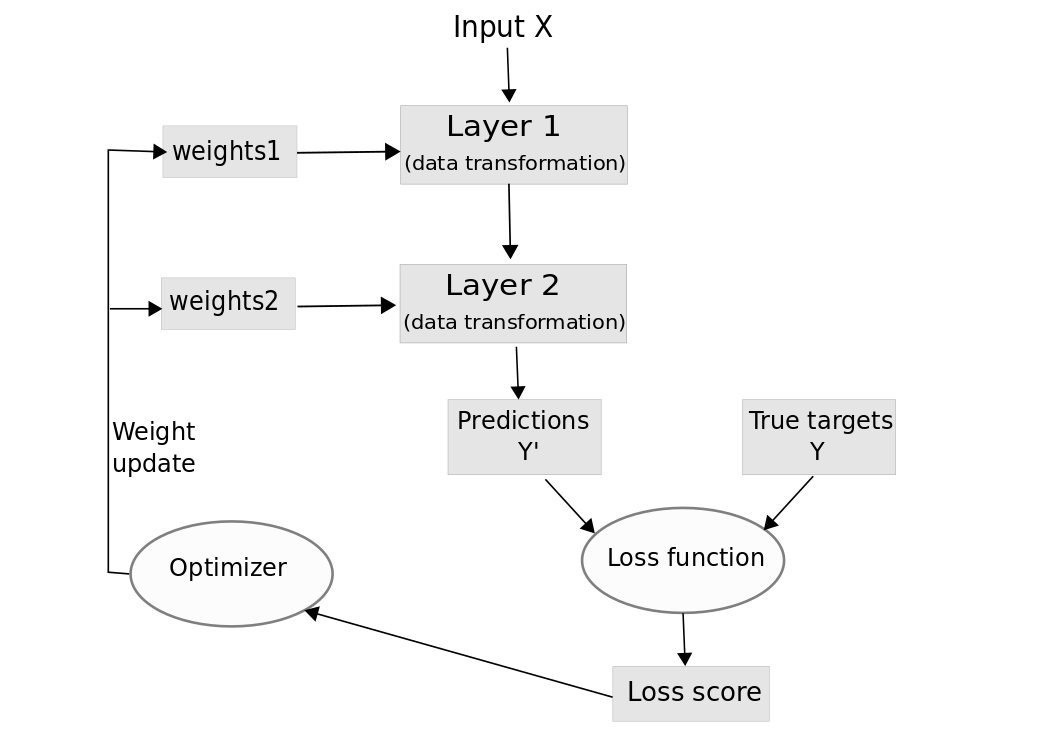
\includegraphics[width=12cm,height=10cm,keepaspectratio]{images/deep_learning_basics.png}
		\caption{Building block of deep learning process }
		\label{fig:deep learning architecture}
	\end{center}
\end{figure}

\subsection{Why data augmentation?}

Deep learning requires a relatively large amount of data and significant computing power to analyze the data. Furthermore, it  requires an efficient algorithm that can calculate hundreds of weights. These requirements posed by deep learning were the significant barriers to the application of deep learning in early 90's. However, nowadays there has been a substantial improvement concerning Central Processing Unit (CPU) and Graphical Processing Unit (GPU). Similarly, digitalization and increasing reach of the internet has generated a significant amount of data. In addition, open source projects contributed by both corporations and researchers in the field of deep learning has streamlined the implementation and deployment of deep learning. As a result of all this, deep learning has been applied to solve various complex problems like image and speech recognition, analyzing particle accelerator data, DNA mutations and autonomous driving with successful results \citep{lecun2015deep}. 

Empirical studies have shown that data representation obtained from deep learning often yield better machine learning results in terms of improved classification modeling \citep{larochelle2009exploring}. Similarly, data generated by a deep learning model is also deemed to be of a better quality than the data generated by generative probabilistic models \citep{najafabadi2015deep}. Compared to conventional machine learning techniques, deep learning technique offers better performance and makes problem-solving simpler by requiring less data engineering and domain expertise. Deep learning is able to capture relevant features of complex problems with the help of multiple representations. Deep learning is simple, scalable, versatile and reusable. It is simple in a sense that it does not require feature engineering which means it removes complex machine learning pipelines with a simple end-to-end trainable models. Thanks to various open source projects, deep learning computation can be parallelized on GPU's or in a distributed system. Deep learning models are trained by iterating over a small batch of data. This batch processing adds the flexibility to train on any size of data. Furthermore, deep learning models are modular allowing the layers from model to be reused to solve similar problems. These pragmatic properties make deep learning functional and useful for researchers and companies alike.    

\section{Data Augmentation in Deep Learning}
Data augmentation has been applied in deep learning with varying degrees of success. The most prominent application of data augmentation has been in image classification, and it has proven to be a successful technique to improve the accuracy of a model \citep{krizhevsky2012imagenet}. Data augmentation can reduce over-fitting as well as make model more robust by introducing artificially generated variables that make the training sample diverse. For example, a recent study on the application of data augmentation in facial recognition showed a significant improvement in the model as a result of data augmentation \citep{kortylewski2018training}. This thesis will primarily go through three data augmentation methods, namely data warping, synthetic minority over-sampling technique, and generative adversarial nets. 

\subsection{Data Warping} 
The most conventional application of data augmentation has been in image classification, and it has proven to be reasonably successful to improve the accuracy of a model. One of the widely used and accepted practices for augmenting image data is to perform geometric and color transformation, such as reflecting an image, cropping and translating the image. Through the application of the various transformation to one image, multiple images can be generated with different perspective and shades. These newly generated images can be used as new training samples. This approach of data augmentation is known as data warping. The term data warping was first used in the context of producing random variations in hand-printed English text data so that new characters are generated mimicking the stylistic variation within and between the writers \citep{yaeger1997effective}.

From its initial application in late 1990 this technique was further extended to improve the performance of a neural network and achieve record performance of the time on MNIST handwritten digit database using a neural network in 2003 \citep{wong2016understanding}. Training data was created by applying simple distortion such as translations, rotation, and skewing. These various transformations helped to create naturally occurring variation as different individuals write letters slightly differently. Augmenting data through the techniques of data warping depends on the problem at hand. Furthermore, these techniques are heuristic in nature which is not guaranteed to be optimal in all situations.

\begin{figure}[ht]
	\begin{center}
		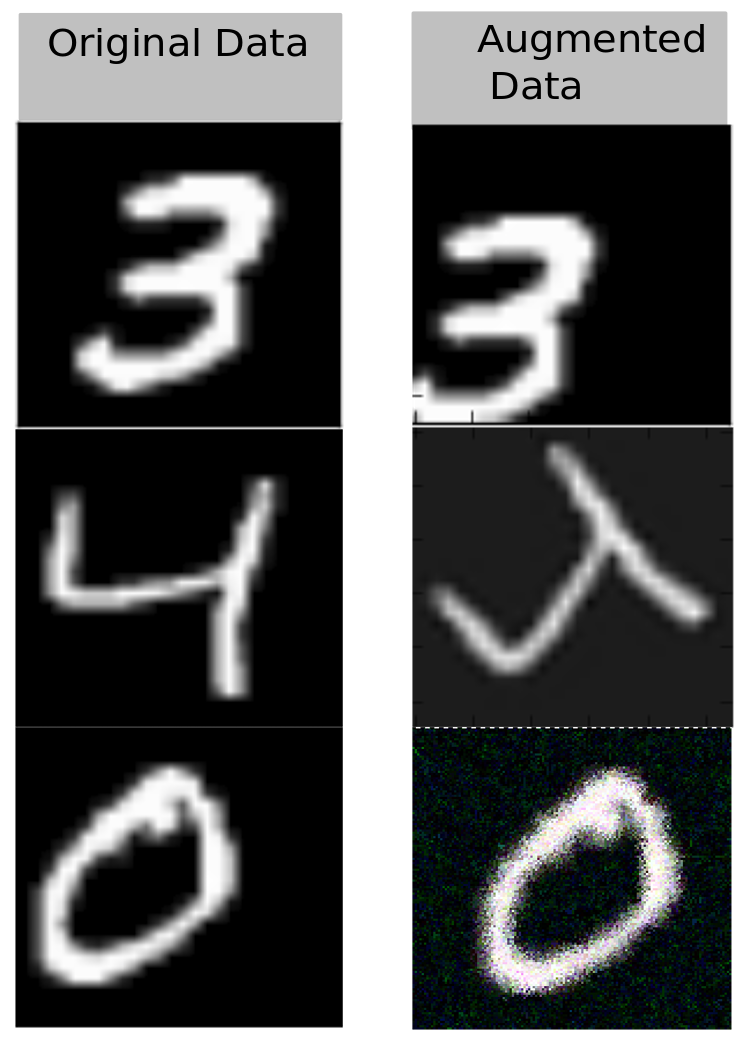
\includegraphics[width=12cm,height=10cm,keepaspectratio]{images/simple_augment_mnist.png}
		\caption{Augmentation via data warping on hand written digits}
		\label{fig:data warping}
	\end{center}
\end{figure} 

The figure ~\ref{fig:data warping} shows the data augmentation applied to image data using various data warping techniques. The top image is warped using a simple random shift of pixels, whereas the bottom image of zero is warped by adding random noise to pixels, and the middle image of four is warped using just a rotation of pixels. This simple technique can make the model more robust. For example by artificially generating several many variation of hand written digit, model can capture naturally occurring variation in hand-writings. This analogy can be extended to the spectral data also, as they can shift slightly up or down due to the variation in concentration or due environmental factors compared to the sample prepared in the lab. Thus, by training model with augmented data model is likely to generalize well in previously unseen measurement data. 

\subsection{SMOTE}
Synthetic Minority Over-Sampling Technique (SMOTE) is a data augmentation technique which is inspired by data warping, particularly its ability to reduce the class imbalance in hand-written digit problems \citep{chawla2002smote}. It is a data augmentation approach in which minority label is over-sampled by creating new synthetic data. This method has been used mainly to address the problem of class imbalance, where real-world data-sets often contain a small percentage of target class examples. The advantage of SMOTE compared to data warping is that synthetic samples are generated in feature space, and this property of SMOTE algorithm makes it application-independent \citep{chawla2002smote}. 

New synthetic samples are obtained from the minority class using the information available in the data. Synthetic samples are generated by taking the difference between feature vector under consideration and its nearest neighbor, then multiplying this difference by a random number between 0 and 1 and finally adding it to the feature vector under consideration \citep{chawla2002smote}. For each sample $x$, the other samples from the same minority class with the smallest Euclidean distance from the $x$ are identified. These other samples are also called as nearest neighbor. One of the nearest neighbors is randomly picked $x^{R}$. The new synthetic sample $S$ is defined in the equation below.

\begin{equation}
S= x + u(x^R -x), where\ u \sim U(0,1) 
% S = x + u.(x^R-x), u ~ U(0,1)
\end{equation} \citep{chawla2002smote} 

Figure ~\ref{fig:SMOTE} succinctly summarizes the synthetic data generation process using SMOTE.

\begin{figure}[ht]
	\begin{center}
		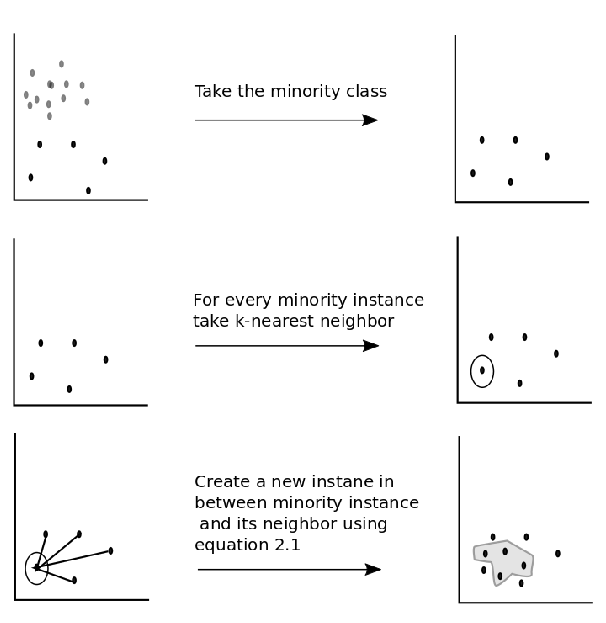
\includegraphics[width=12cm,height=10cm,keepaspectratio]{images/SMOTE_2.png}
		\caption{Synthetic data generation using SMOTE}
		\label{fig:SMOTE}
	\end{center}
\end{figure} 

One alternative to SMOTE is to over-sample the minority class with replacement. Some previous study has shown that while this practice can increase the number of samples in training set, it does not significantly increase the class recognition of minority class \citep{chawla2002smote}. In the experiment conducted by \citet{chawla2002smote}; when the minority class was over-sampled by increasing amounts, the decision tree tried to identify similar but more specific regions in the feature space of minority class. In other words, the replication of same data causes the model to focus on those repeated samples and also to over-fit the data. Over-sampling the minority class with replacement can produce an undesired result of shrinking the decision boundary for minority class. Ideally, we would want to increase the decision boundary of minority class so that it generalizes well for unseen data. In the same paper, \citet{chawla2002smote} demonstrated that SMOTE approach could improve the accuracy of the classifier for a minority class by applying it on various imbalanced data-sets.

\subsection{Generative Adversarial Nets}
One of the promising techniques of data augmentation in the field of deep learning is Generative Adversarial Nets (GANs). It is a powerful technique to generate data. GANs uses a min-max strategy where one neural net successively generates counterfeit samples from the original data distribution in order to fool the other net, and the other net is then trained to better distinguish the counterfeits \citep{goodfellow2014generative}. There are two main elements of a GANs: Generator and Discriminator. The objective of the generator is to take a random input and generate a sample data, whereas the objective of the discriminator is to take input from the original data or data generated from generator and to predict whether the input is real or generated. Discriminator aims to maximize the probability of assigning the correct label to both original sample and the counterfeit, whereas generator simultaneously aims to minimize the difference between original and counterfeit samples \citep{goodfellow2014generative}. In this sense, the discriminator and generator play a two-player mini-max game. The generator obtained from this process can be used to generate synthetic samples of data which closely represents the actual data. The figure below illustrates the GANs architecture.

\begin{figure}[ht]
	\begin{center}
		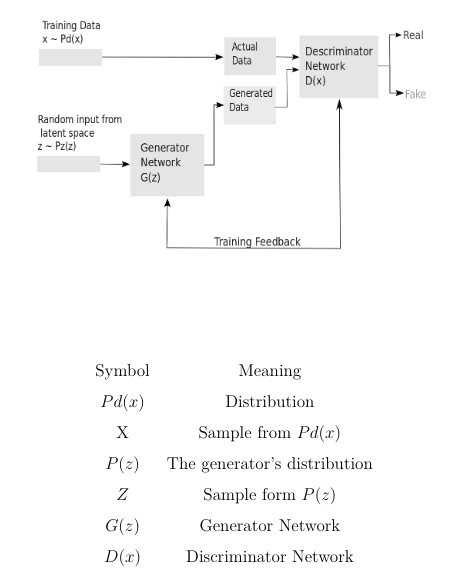
\includegraphics[width=12cm,height=13cm,keepaspectratio]{images/GAN_3.png}
		\caption{GANs architecture}
		\label{fig:GAN}
	\end{center}
\end{figure} 

%\begin{center}
%	\begin{tabular}{ c c }
%		Symbol & Meaning  \\ 
%		$Pd(x)$ & Distribution \\ 
%		X & Sample from $Pd(x)$  \\  
%		$P(z)$ & The generator's distribution \\  
%		$Z$ & Sample from $P(z)$ \\      
%		$G(z)$ & Generator Network \\  
%		$D(x)$ & Discriminator Network 
%		
%	\end{tabular}\\
%\end{center}


Here, generator $G(z)$ takes an input from $P(z)$. The generated data is supplied to discriminator network along with the actual data. The discriminator takes input $x$ from $Pd(x)$ where $Pd(x)$ is the real distribution, $D(x)$ then solves a binary classification problem. Two models compete against each other which ideally leads to the generator being able to produce fairly real looking samples from $P(z)$. This process can be mathematically represented as:

\begin{equation}
min_{G}max_{D}L(D,G) = E_{x \sim Pdata(x)}[logD(x)]+E_{z \sim P_{z}(z)}[log(1-D(G(z)))]
\end{equation} 
\citep{goodfellow2014generative}

In equation 2.2 first term is entropy that the data from real distribution $P_d$ passes through the discriminator. We want to maximize discriminator given real data $P_{d}(x)$ by maximizing $E_{x_{d}(x)}[logD(x)]$. Meanwhile given fake data $P_{(z)}$ the discriminator is expected to output a probability of $D(G(z))$ close to zero by maximizing second part of equation $E_{z~P_{z}(z)}[log(1-D(G(z)))$. Whereas, the generator is trained to increase the chances of $D(x)$ producing a high probability for a fake example, thus to minimize $E_{z~P_{z}(z)}[log(1-D(G(z)))$.

GANs has been extensively used in machine learning applications such as computer vision and image recognition. GANs have been useful even with relatively small sets of data as one can use a transfer learning technique. GANs have been used for example to train a self-driving car to drive in the night or rain using only data collected on a sunny day \citep{gurumurthy2017deligan}. Recently there have been many studies in the application of GANs in medical diagnosis mainly to augment the medical imaging data. Medical industry also faces the problem of limited data, as data is heavily regulated and costly to acquire. In one recent study conducted by \citet{frid2018synthetic}, authors successfully used GANs to augment the limited medical image data to improve a deep learning model. Using GANs as augmentation method authors were able to gain 7 percent improvement in accuracy over the traditional augmentation methods like data warping. 

GANs offer a unique proposition in data augmentation. Unlike data warping, instead of figuring out augmentation that is label invariant we let the deep learning model to find the label invariant augmentation. Thus, the expectation from the GANs model is that the data is generated from the actual data distribution so that the newly generated data has the core characteristics of real data.   

\section{Model Evaluation}

Since the thesis tries to evaluate the performance of various deep learning models, metrics for model assessments needs to be clearly laid out. Model evaluation depends on the type of problem model is trying to solve. Machine learning divides classification problem into binary, multi-class, multi-labeled and hierarchical tasks \citep{sokolova2009systematic}. The classification problem tackled in this thesis falls under the multi-class classification problem. Formally multi-class problem is defined as a classification problem where the input is to be classified into one and only one, of 'l' non-overlapping classes \citep{sokolova2009systematic}.

Empirical evaluation remains the most used approach for the model assessment \citep{sokolova2009systematic}. The empirical comparison is made through applying algorithms from the model on data-sets that are not used for model training and then evaluating the performance of the classifiers that the algorithms have produced. Often accuracy remains the most used evaluation measure for evaluating models \citep{sokolova2009systematic}. However, accuracy is not the only measure for performance evaluation. The performance of a classification algorithm from given model can also be evaluated by dividing the accuracy into smaller components. For instance, computing the number of correctly recognized class examples (true positives), the number of correctly recognized examples that do not belong to the class (true negatives), and examples that either were incorrectly assigned to the class (false positives) or that were not recognized as class examples (false negatives) \citep{sokolova2009systematic}. These four values constitute a confusion matrix shown in the table ~\ref{table:Confusion matrix}.



\begin{table}[ht]
	\centering
	\caption{Confusion matrix for binary classification }
	% Place the label just after the caption to make the link work
	\label{table:Confusion matrix}
	\begin{tabular}{|p{3cm}|p{4cm}|p{4cm}|} 
		% Alignment of sells: l=left, c=center, r=right. 
		% If you want wrapping lines, use p{width} exact cell widths.
		% If you want vertical lines between columns, write | above between the letters
		% Horizontal lines are generated with the \hline command:
		\hline
		\textbf{Data class} & \textbf{Classified as pos}& \textbf{Classified as neg}\\ 
		\hline % The line on top of the table
		\textbf{pos} & true positive (tp) & false negative (fn) \\ 
		\textbf{neg} & false positive (fp) & true negative (tn)  \\ 
		
		% Place a & between the columns
		% In the end of the line, use two backslashes \\ to break the line,
		% then place a \hline to make a horizontal line below the row 
		
		\hline		
	\end{tabular} % for really simple tables, you can just use tabular
	% You can place the caption either below (like here) or above the table
	
\end{table} % table makes


Accuracy is just a proportion of the total number of prediction that was correct. Precision and recall provided more insight than just the overall accuracy. To use the analogy of cancer diagnosis problem: precision tells what proportion of patients diagnosed by the model as having cancer had cancer whereas recall tells what proportion of patient that actually had cancer was diagnosed by the model as having cancer. What precision and recall do is they break the accuracy into small metrics like true positive, false positive and false negative. Precision is defined as the number of true positives over the number of true positives plus the number of false positives. Recall is defined as the number of true positives over the number of true positives plus the number of false negatives \citep{scikit-learn}. Furthermore, often precision and recall are expressed in one number which is its weighted average known as the F1 score. In other words F1 score is just the harmonic mean of precision and recall.

\begin{equation}Accuracy = \dfrac{TP + TN}{TP+TN+FP+FN}\end{equation} 
\begin{equation}Precision = \dfrac{TP}{TP+FP}\end{equation} 
\begin{equation}Recall = \dfrac{TP}{TP+FN}\end{equation} 
\begin{equation}F1 = \dfrac{2 (recall \times precision) }{recall+precision}\end{equation} 

The above metrics are expressly designed for the binary classification task, where the input is to be classified into one, and only one, of two non-overlapping classes \citep{sokolova2009systematic}. However, these binary metrics can be easily extended to the multi-class problem. There is a number of ways to average binary metric calculations across the set of classes. One way to averaging binary metric is macro averaging. Macro averaging calculates the mean of the binary metrics, giving equal weight to each class. In problems where infrequent classes are important, macro-averaging can be a means of highlighting their performance \citep{scikit-learn}.

\begin{equation}Precision_M =  \dfrac{\sum^l_i\dfrac{tp_i}{tp_i+fp_i}}{l} \end{equation} 
\begin{equation}Recall_M =  \dfrac{\sum^l_i\dfrac{tp_i}{tp_i+fn_i}}{l} \end{equation} 
\begin{equation}Fscore_M =  \dfrac{2 (Precision_M \times Recall_M) }{Precision_M+Recall_M }\end{equation}

To summarize, there are various metrics for evaluation of classification models. For a multi-class classification problem, model metrics are merely the extension from binary classification metrics. It is often the case that no single metrics can comprehensively measure and evaluate the quality of the model. Therefore depending on the application of model, relevant application metrics needs to be used. In this thesis, macro-averaging is used to evaluate the models, as this approach will emphasize the quality of the model based not only on the accuracy of majority class but also based on infrequent minority classes.

